%*****************************************
\chapter{Evaluation}\label{ch:evaluation}
%*****************************************

\section{Evaluation FOL}
\label{sect:evaluation-fol}

We describe our experience with applying our approach to the reconstruction of SMT proofs to benchmark problems collected from the SMT-LIB library and from the TLAPS proof assistant.

\subsection{Parallel reconstruction and checking optimizations}
\label{ssec:parallel}

In order to speed up the checking of Alethe proofs in Lambdapi, we can take advantage of multiprocess execution.
This is possible because there are no cyclic dependencies between steps in Alethe proof traces, so one can assume all hypotheses $h$ used in a proof of step $t$ and check their proofs independently.
In practice, we divide the proof trace into files that contains at most a fixed number of steps and include in each of them the hypotheses of previous files as axioms.

In addition, to reduce the memory usage and checking time, we define a constant for any closed subterm that is used more than once in the Alethe proof trace.
This is similar to the \kw{:named} attribute of SMT-LIB used by solvers.

\subsection{Benchmarks}

Our benchmark \cref{tab:benchmarks-description} is composed of files from the SMT-LIB benchmarks\footnote{\url{https://smtlib.cs.uiowa.edu/benchmarks.shtml}} of \kw{QF\_UF} and \kw{UF} theories, and additional proof obligations from the SMT backend of the TLAPS proof system.
Our work is aimed at reconstructing proofs found by SMT solvers called by proof assistants such as Coq, Isabelle, Rodin or TLAPS. One particular goal of our development is the reconstruction of theorems expressed in the set theory of TLA\textsuperscript{+} (i.e., not involving temporal logic) in Lambdapi.
TLA\textsuperscript{+} \cite{lamport:specifying} is a language based on set theory and linear-time temporal logic for formally specifying and verifying systems, particularly concurrent and distributed algorithms.
Its interactive proof environment TLAPS \cite{tla-proofs} relies on users guiding the proof effort; it integrates automatic backends, including SMT solvers, to discharge proof obligations \cite{smttlaps, ABZrosalie}. TLAPS encodes set theory as \kw{UF} constraints, which makes this SMT-LIB theory an attractive target for our work. Support of arithmetic reasoning is left as future work.

\begin{table}%[tb]%[H]
    \begin{tabular}{|l c c c c c c|}
    \hline
    Name & Logic & Samples & Steps & Elaborated & Translated & Checked \\
    \hline
    sledgehammer & UF & 1403 & 1/143/2301 & 1226 & 1209 & 994 \\
    allocator & UFNIA & 38 & 5/107/810 & 38 & 38 & 38 \\
    eq\_diamond & QF{\_}UF & 100 & 9/686/3579 & 100  & 100 & 74 \\
    2018-Goel-hwbench & QF{\_}UF & 229 & 12/166/83149 & 213 & 192 & 160\\
    EWD840 & UFNIA & 19 & 9/140/1000 & 19 & 19 & 11 \\
    20170829-Rodin & QF{\_}UF & 20 & 1/13/107 &  20 & 20 & 16\\
    \hline
    \end{tabular}
    \caption{Benchmark samples.}
    \label{tab:benchmarks-description}
\end{table}

We therefore chose samples related to proof assistants in the SMT-LIB benchmarks, e.g. Sledgehammer, and we have two benchmarks from TLA\textsuperscript{+} community modules.
The Allocator module \cite{allocator} is a case study for the specification and analysis of reactive systems in TLA\textsuperscript{+}. EWD840 \cite{ewd840} formalizes a termination detection algorithm for distributed computations due to Dijkstra.

\cref{tab:benchmarks-description} contains the details and results of each group of benchmarks.
The column \emph{Samples} describes the number of problems available with status \emph{unsat}. 
The column \emph{Steps} indicates the smallest, average and largest number of steps that appear in the proof traces of the samples in the group, excluding \kw{assume} steps.
For example, the \emph{2018-Goel-hwbench} collection contains proof traces varying between 12 to 83149 steps, with 166 steps on average.
We only reconstruct proof traces that can be handled by Carcara.
The column \emph{Elaborated} indicates the number of proof traces checked and elaborated by Carcara.
The column \emph{Translated} indicates the number of elaborated proof that can be translated into a Lambdapi proof.
The remaining proof traces could not be reconstructed due to limitations in our current work, mainly due to unsupported Alethe commands.
The column \emph{Checked} gives the number of proof traces for which a Lambdapi proof could be constructed.
We did not impose a time restriction for the Carcara elaboration and our translation because that time is negligibly small.
However, we set a timeout of 20 seconds for Lambdapi to check the proof.
The parallel checking described in \cref{ssec:parallel} is used only on proof traces with more than 3000 steps (excluding \kw{assume}). 

To evaluate the impact of elaboration on the proof size, we measured the number of steps of each proof before and after elaboration, as well as the number of steps of each relevant rule (namely \texttt{resolution}, \texttt{contraction} and \texttt{reordering}). \cref{tab:elaboration-impact} shows these results. The average number of steps increased moderately with elaboration, as did the fraction of \texttt{resolution} and \texttt{contraction} steps, which is an expected effect from the elaboration of \texttt{resolution} steps. As expected, all \texttt{reordering} steps were eliminated.

\begin{table}%[tb]%[H]
    \begin{tabular}{|l c c c c|}
    \hline
    & Average number of steps & \texttt{resolution} & \texttt{contraction} & \texttt{reordering} \\ \hline
    Original   & 21093.89 & 18.39 \% & 3.31 \% & 3.61 \% \\
    Elaborated & 26160.01 & 20.82 \% & 6.53 \% & 0.00 \% \\
    \hline
    \end{tabular}
    \caption{Average number of steps before and after elaboration, and the proportion of these steps that use each of the relevant rules.}
    \label{tab:elaboration-impact}
\end{table}

The boxes in \cref{fig:benchmarks-graph} are plotted as $log(1 + time)$  to make them comparable. But in y-axis we present the original values of $time$ for readability.
In \cref{tab:benchmarks-times} and \cref{fig:benchmarks-graph}, we can observe that the majority of reconstructed proofs can be checked by Lambdapi in a few milliseconds and less than 3 seconds (red line in \cref{fig:benchmarks-graph}).
%We intend to include our work in proof assistants such as TLAPS, so we seek a tolerable reconstruction time. 
Some samples cannot be reconstructed because some simple deduction and RARE rules are not yet implemented. 
Other samples cannot be reconstructed because some rules that expect a number of parameters such as $\kw{cong}_n$ or $\kw{subproof}_n$  are not yet defined, for example
samples in $\kw{eq\_diamond}$ failed because the lemma $\kw{subproof\_98}$ is not defined. We are considering to review this rule to make it scale.
Moreover, nested \kw{bind} rules can make the proof reconstruction fail in EWD840 or 2018-Goel-hwbench because there is a naming collision with fresh variables introduced in the context. We plan to fix this problem by reviewing our generation of variable names.
We should be able to increase the number of proofs reconstructed in these categories with little effort.
Some RARE rules failed to reconstruct because Lambdapi is not able to infer some implicit arguments. We have to modify the proof generated by giving explicitly some arguments.
Concerning the large proofs in 2018-Goel-hwbench, use of the technique described in \cref{ssec:parallel} allows us to reconstruct some, but not all parts of the proof, and we consider it a failed case.
Although these do not appear in \cref{fig:benchmarks-graph} and \cref{tab:benchmarks-times}, we have been able to manually adjust some large proofs (of 10-30k lines) and have them checked within 2 seconds with parallel processing.
For benchmarks using the LIA (sub-)logic, we only reconstruct those proof steps where arithmetic reasoning does not play an essential role (beyond simplification).
Some samples take more than 3 seconds to be certified. We suspected, and this has been confirmed by the authors of Lambdapi, that there is a bottleneck in the unification of AC terms.

\begin{figure}
    \centering
    \begin{tikzpicture}
    \begin{axis}[
        xtick={1,2,3,4,5,6},
        yticklabels={0, 0.50, 2, 4, 10},
        ytick={0, 0.17, 0.5, 0.7, 1.04},
        xticklabels={sledge, alloc, eq, goel, ewd, rodin},
        ylabel={Time (s)},
        boxplot/draw direction=y,
        /pgfplots/boxplot/box extend=0.3
        ]
        % Sledge
        \addplot+ [boxplot prepared={lower whisker=0.055, lower quartile=0.094, median=0.178,
        upper quartile=0.397, upper whisker=2.825},] table[row sep=\\,y index=0] {\\};
    
        % Alloc
        \addplot+ [boxplot prepared={lower whisker=0.055, lower quartile=0.065, median=0.138,
        upper quartile=0.343, upper whisker=2.075},] table[row sep=\\,y index=0] {\\};
    
        % Eq
        \addplot+ [boxplot prepared={lower whisker=0.055, lower quartile=0.108, median=0.180,
        upper quartile=0.291, upper whisker=1.1448},] table[row sep=\\,y index=0] {\\};
    
         % Goel
         \addplot+ [boxplot prepared={lower whisker=0.057, lower quartile=0.065, median=0.069,
         upper quartile=0.119, upper whisker=1.012},] table[row sep=\\,y index=0] {\\};
    
        % Ewd
        \addplot+ [boxplot prepared={lower whisker=0.058, lower quartile=0.078, median=0.086,
        upper quartile=0.110, upper whisker=0.925},] table[row sep=\\,y index=0] {\\};
    
        % Rodin
        \addplot+ [boxplot prepared={lower whisker=0.053, lower quartile=0.055, median=0.057,
        upper quartile=0.060, upper whisker=0.076},] table[row sep=\\,y index=0] {\\};
    
        \draw[red] (axis cs:0,0.6) -- (axis cs:7,0.6); % Comfort line
    \end{axis}
    \end{tikzpicture}
    \caption{Checking time variations between samples.}
    \label{fig:benchmarks-graph}
\end{figure}

\begin{table}%[tb]%[H]
    \begin{tabular}{|l c c c c c |}
    \hline
    Name & Min & Q1 & Mean & Q3 & Max \\
    \hline
    sledgehammer & 56 & 98 & 195 & 487 & 15853  \\
    allocator & 56 & 67 & 148 & 408 & 6967 \\
    eq\_diamond & 57 & 114 & 196 & 337 & 3254 \\
    2018-Goel-hwbench & 58 & 66 & 71 & 126 & 1751 \\
    EWD840 & 59 & 81 & 89 & 116 & 1522  \\
    20170829-Rodin & 54 & 56 & 58 & 61 & 79  \\
    \hline
    \end{tabular}
    \caption{Lambdapi checking times in milliseconds.}
    \label{tab:benchmarks-times}
\end{table}


Our work revealed that some proof obligations in Allocator initially failed to be reconstructed. In fact, the proof trace found by the SMT solver became incorrect after elaboration by Carcara. This allowed us to detect multiple bugs in the Carcara elaborator, which have since been corrected.
Moreover, one reconstruction failure was due to one of the set theory axioms of TLA\textsuperscript{+} being incorrectly encoded in SMT, and this issue has also been fixed.
Compared to our previous work \cite{ColtellacciMD24}, we have been able to significantly increase the number of proofs that can be reconstructed, as well as the efficiency of reconstruction.




\section{Evaluation LIA}
\label{sec:evaluation-lia}

\begin{table}[t]
\centering
\begin{tabular}{|c|c|c|c|c|c|c|}
\hline                                                             % Succ - Err -Timeout   % Succ - Error        % Succ - Err - Timeout % Succ - Err - Timeout
\textbf{Logic}                & \textbf{Bench}  & \textbf{Samples} & \textbf{Proofs}       & \textbf{Elaborate} & \textbf{Translate} & \textbf{Check} \\ \hline
\multirow{4}{*}{\tt{LIA}}     & tptp            & 36               &  36 - 0 - 0           &  36 - 0             & 36 - 0 - 0          & 28 - 8 - 0       \\ \cline{2-7} 
                              & Ultimate        & 153              &  120 - 0 - 33         &  73 - 80            & 68 - 5 - 0          & 50 - 18 - 0      \\ \cline{2-7} 
                              & Svcomp'19      & 27               &  27 - 0 - 0           &  25 - 2             & 0 - 25 - 0          & 0                \\ \cline{2-7} 
                              & psyco           & 50               &  48 - 0 - 2           &  48 - 2             & 43 - 0 - 5          & 0 - 39 - 6       \\ \hline
\multirow{2}{*}{\tt{QFLIA}}   & SMPT            & 1568             &  1501 - 67 - 0        &  1491 - 32          & 1470 - 0 - 21       & 804 - 638 - 34   \\ \cline{2-7}
                              & rings           & 294              &  63 - 0 - 231         &  49 - 21            & 49 - 0 - 0          & 7 - 0 - 42       \\ \cline{2-7} 
                              & CAV2009       & 85               &  85 - 0 - 0           &  19 - 0             & 19 - 0 - 0          & 19 - 0 - 0       \\ \hline
\multirow{2}{*}{\tt{UFLIA}}   & sledgeh    & 1521             &  1343 - 0 - 178       &  1278 - 222         & 1258 - 13 - 7       & 713 - 467 - 80   \\ \cline{2-7} 
                              & tokeneer        & 1732             &  1732 - 0 - 0         & 1689 - 43           & 1689 - 0 - 0        & 1482 - 197 - 10  \\ \hline
\end{tabular}
\caption{Benchmark results.}
\label{table:benchmarks-description}
\end{table}

Our benchmark suite, \cref{table:benchmarks-description} is composed of files from the SMT-LIB benchmarks\footnote{\url{https://smtlib.cs.uiowa.edu/benchmarks.shtml}}.
The suite includes a total of 5,466 samples drawn from 9 benchmarks spanning 3 SMT-LIB logics: \texttt{LIA}, \texttt{QFLIA}, and \texttt{UFLIA} that correspond to those covered by our method.
%These were selected because our previous work supported the \texttt{QF} and \texttt{UF} fragments.
Within the logics \texttt{QFLIA} and \texttt{UFLIA}, we prioritized benchmarks with the most significant number of available samples.
Table~\ref{table:benchmarks-description} provides a detailed breakdown of the benchmarks and corresponding results.
The \emph{Logic} column indicates the SMT theory used, while the \emph{Bench} column lists abbreviated benchmark names.
The column \emph{Samples} describes the number of problems available with status \emph{unsat}. 
Each of the columns \emph{Proofs}, \emph{Translate}, and \emph{Check} reports a triple in the format \tt{success - error - timeout}, representing respectively the number of successful executions, failed attempts, and timeouts. 
The \emph{Proofs} column reports the number of proofs generated by cvc5\footnote{cvc5 version 1.2.1-dev.144.38fcc340e5 [git 38fcc340e5 on branch main]} that do not contain \lstinline[language=SMT,basicstyle=\ttfamily\footnotesize]|to_real| cast operator.
The \emph{Elaborate} column shows a pair of values: the number of proofs that were successfully elaborated by Carcara, and the number that failed. Only proofs successfully elaborated by Carcara are considered for translation.
The \emph{Translate} column gives the number of proof traces successfully translated into Lambdapi proofs, while the \emph{Check} column indicates the number of these translated proofs that were successfully type-checked by Lambdapi. 

We enforced a timeout of 30 seconds for cvc5 to find a proof and 30 seconds for the translation step with Carcara.
No timeout was imposed during the elaboration step, as the runtime is negligible.
A timeout of 20 seconds was set for Lambdapi when type-checking the final proofs to ensure that proof verification remains as fast as possible.\footnote{All benchmarks were executed in parallel using GNU parallel \cite{tange_2025_15071920} with an Apple silicon M2.} % Ask by the tool to be cited

All nine benchmarks demonstrated consistently reliable proof generation, with few or no timeouts, except for the \emph{rings} benchmark.
The elaboration phase was generally robust, except in the \emph{Ultimate} benchmark, where an error in the elaborator caused failures.
For \texttt{LIA}, performance in the translation and checking stages was mixed. In particular, for \emph{Svcomp'19} and \emph{psyco}, no or few proofs could be translated or verified, mainly due to currently unsupported simplification rules involving the \texttt{ite} operator.
The \texttt{QFLIA} benchmarks exhibited more reliable proof checking in \emph{SMPT} and \emph{CAV2009}, while only a small number of proofs from the \emph{rings} benchmark were successfully checked.
The errors encountered during the elaboration of the \emph{CAV2009} come from a bug in the elaborator. Since the samples in this benchmark are derived from a common base problem while increasing in size, the bug propagated across all samples that depend on the same base instance.
For \emph{rings}, this limitation is due to the presence of \texttt{la\_generic} terms with hundreds of uninterpreted variables; the current normalization mechanism, described in \cref{ssec:normalization}, relies on a built-in term ordering that is not sufficiently efficient in this setting.
Benchmarks under \texttt{UFLIA} performed better throughout the pipeline. Most proofs were successfully generated and elaborated, and a large portion were translated and verified by Lambdapi, particularly in the \emph{tokeneer} dataset.
The higher number of errors in \emph{SMPT} and \emph{sledgeh} is primarily due to unsupported RARE rules related to \tt{QF\_UF} logic, as well as unhandled cases in the \texttt{evaluate} rule for \texttt{LIA} and \texttt{QF\_UF}.

\begin{table}[t]
\centering
\begin{tabular}{|c|c|c|c|c|c|}
\hline
\textbf{Bench}      & \textbf{Min} & \textbf{Q1} & \textbf{Mean} & \textbf{Q3} & \textbf{Max} \\ \hline
tptp                & 240          & 262         & 263           & 267         & 336          \\ \hline
Ultimate            & 82           & 96          & 100           & 111         & 346          \\ \hline
SMPT                & 52           & 55          & 55            & 56          & 293          \\ \hline
rings               & 670          & 704         & 773           & 826         & 1197         \\ \hline
CAV2009           & 54           & 296         & 403           & 498         & 683          \\ \hline
sledgeh             & 53           & 166         & 354           & 552         & 1594         \\ \hline
tokeneer            & 55           & 60          & 61            & 248         & 753          \\ \hline
\end{tabular}
\caption{Lambdapi checking times in milliseconds.}
\label{table:benchmarks-list}
\end{table}

Table~\ref{table:benchmarks-list} reports the Lambdapi proof-checking times in milliseconds, presenting the minimum, first quartile (Q1), mean, third quartile (Q3), and maximum durations for each benchmark.
In most cases, the checking time remains below one second.
% , with the exception of a few outliers particularly in the \emph{sledgehammer} and \emph{rings} benchmarks that exhibit higher upper tails.


\section{Validating \texorpdfstring{\tlaplus} SMT proof}\label{sec:tla-eval}

\begin{figure}[tb]
    \centering
    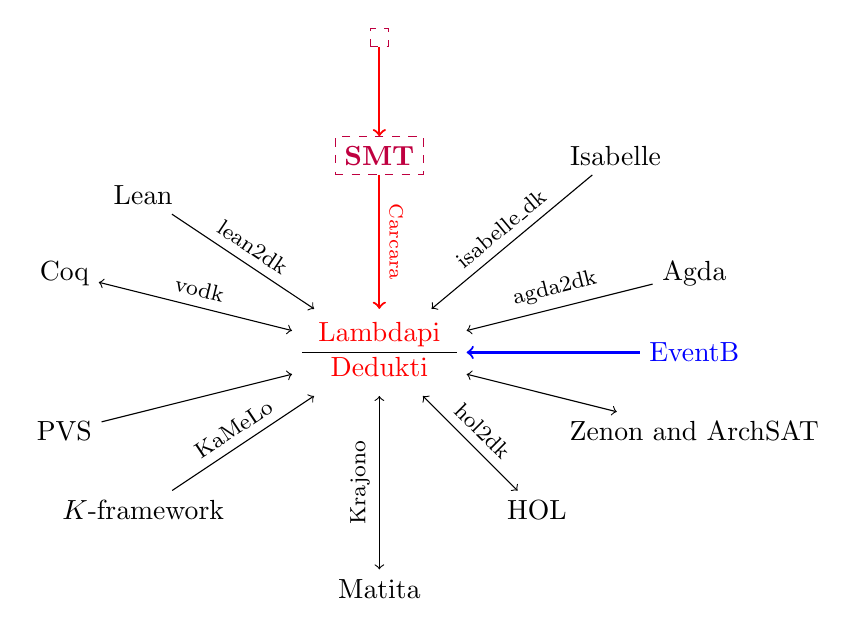
\begin{tikzpicture}
      \path (0,0) node (lp) {\begin{tabular}{c}
        \textcolor{red}{Lambdapi} \\
        \hline
        \textcolor{red}{Dedukti}
      \end{tabular}}
            (-4,1) node (coq) {Coq}
            (-3,2) node (lean) {Lean}
            (0,2.5) node [draw, dashed, purple] (smt) {\color{purple}\textbf{SMT}}
            (0,4) node [draw, dashed, purple] (tla) {\color{purple}\tlaplus}
            (3,2.5) node (isa) {Isabelle}
            (4,1) node (agda) {Agda}
            (-3,-2) node (k) {$\mathbb{K}$-framework}
            (0,-3) node (mat) {Matita}
            (2,-2) node (hol) {HOL}
            (-4,-1) node (pvs) {PVS}
            (4,0) node (eventb) {\textcolor{blue}{EventB}}
            (4,-1) node (ze) {Zenon and ArchSAT}
            ;
      \draw[->,red, thick] (smt) -- (lp) node[midway,sloped,above]
      {\scriptsize{Carcara}};
      \draw[->,red, thick] (tla) -- (smt) node[midway,sloped,above] {};
      \draw[->,blue, thick] (eventb) -- (lp) node[midway,sloped,above] {};
      \draw[->] (lean) -- (lp) node[midway,sloped,above] {\footnotesize{lean2dk}};
      \draw[->] (isa) -- (lp) node[midway,sloped,above] {\footnotesize{isabelle\_dk}};
      \draw[->] (agda) -- (lp) node[midway,sloped,above] {\footnotesize{agda2dk}};
      \draw[<->] (ze) -- (lp) node[midway,sloped,above] {};
      \draw[<->] (hol) -- (lp) node[midway,sloped,above] {\footnotesize{hol2dk}};
      \draw[<->] (mat) -- (lp) node[midway,sloped,above] {\footnotesize{Krajono}};
      \draw[->] (pvs) -- (lp);
      \draw[->] (k) -- (lp) node[midway,sloped,above] {\footnotesize{KaMeLo}};
      \draw[<->] (coq) -- (lp)  node[midway,sloped,above] {\footnotesize{vodk}};
    \end{tikzpicture}
    \caption{Verifying TLAPS proof with Lambdapi.}
    \label{fig:interop-tla}
\end{figure}


Following our approach, we collect the Alethe proof produced by the SMT solver and reconstruct it in Lambdapi.
However, we do not currently re-integrate the reconstructed proof back into \tlaplus.
Supporting this step would be important to ensure that the reconstruction indeed corresponds to the original theorem stated in \tlaplus, particularly because the SMT encoding produced by the backend has not yet been fully formalized.
Moreover, since the SMT solver performs \emph{skolemization} during preprocessing, recovering the original problem would require an additional \emph{deskolemization} phase \cite{desko}.
In the absence of this feedback mechanism, the reconstruction provides an additional but still partial layer of assurance.


\subsection{Reconstruction integrated to the Toolbox}
\label{ssec:tlaps-toolbox}

TODO

\subsection{Evaluation of TLAPS reconstruction}
\label{ssec:tlaps-evaluation-results}

TODO